\documentclass[../main/main.tex]{subfiles}

\begin{document}

\newpage
\chapter{Testing}

\section{Iterative Testing}
I have been playtesting the program throughout the development process to find any bugs and fix them accordingly. However, a few issues have required additional measures.

\subsection{Minimax}
Since minimax is recursive algorithm, debugging it has proven a challenge. I have therefore configured the Python \lstinline{logging} library to help collect information on the minimax tree for every function call.

\noindent\verb|base.py|
\lstinputlisting[firstline=27, lastline=51, caption=BaseCPU Method for logging minimax statistics]{../../data/states/game/cpu/base.py}

\subsection{Migrations}
To correct errors made to the \lstinline{games} table, since recreating it would mean deleting all existing games, I have opted to use migrations to fix bugs by editing the table schema, as shown in Section \ref{sec:migrations}.

\section{Unit Tests}
\subsection{Board Evaluator}
To test every aspect of the evaluation function, I have set up some unit tests with custom positions using my editor screen. These positions are designed to test every aspect of the evaluation, along with some obviously imbalanced positions to test the overall accuracy of the evaluation function. All positions are set up to give an advantage to the blue player.

\begin{longtable}[c]{l|l|l|l}
    \toprule
    \textbf{Evaluating} & \textbf{FEN string} & \textbf{Score} & \textbf{Passed}\\
    \midrule
    \endfirsthead
    \endhead

    Material & \verb|sc9/10/10/4paPa4/5Pa4/10/10/9Sa b| & 124 & \checkmark\\
    Position & \verb|sc9/4nanana3/10/10/10/4NaNaNa3/10/9Sa b| & 66 & \checkmark\\
    Mobility & See footnote\footnote{scpapa7/papapa7/papapa1Pa1Pa1Pa1/10/4Pa1Pa1Pa1/10/4Pa1Pa3/9Sa b} & 196 & \checkmark\\
    King Safety & \verb|sc4fa3pa/10/10/10/10/10/10/5FaPa2Sa b| & 3 & \checkmark\\
    Combined & See footnote\footnote{scnc1fcncpbpb3/pa9/pb1pc1rbpa3Pd/1Pc2Pd4Pc/2Pd1RaRb4/10/7Pa2/2PdNaFaNa3Sa b} & 437 & \checkmark\\

    \bottomrule
    
\caption{Board evaluator test results}
\label{tab:testing-evaluator}
\end{longtable}


\subsection{CPU}
Similarly, to evaluate the strength of my CPU, I have setup some custom positions that I already know the best continuation of, and run each CPU engine on them to test if they can solve it.

sc9/pafa8/Fa9/10/10/10/10/9Sa b

I have also personally played against the CPU engines to gauge its strength in a realistic setting. The results are shown below:

\begin{longtable}[c]{c|c}
    \toprule
    \textbf{Me} & \textbf{CPU}\\
    \midrule
    \endfirsthead
    \endhead

    2 & 5\\

    \bottomrule
    
\caption{Score of me vs CPU (I am very bad)}
\label{tab:me-cpu}
\end{longtable}

\begin{longtable}[c]{c|c}
    \toprule
    \textbf{Mr Myslov} & \textbf{CPU}\\
    \midrule
    \endfirsthead
    \endhead

    1 & 6\\

    \bottomrule
    
\caption{Score of Mr Myslov vs CPU (Mr Myslov is even worse)}
\label{tab:myslov-cpu}
\end{longtable}

\subsection{Shadow Mapping}
To test the shadow mapping algorithm, I have set up some occluding objects togehter with a light source. Since visuals are subjective, me and my client have deemed the following results to be adequate.

\begin{figure}[H]
    \centering

    \begin{subfigure}[b]{0.3\columnwidth}
    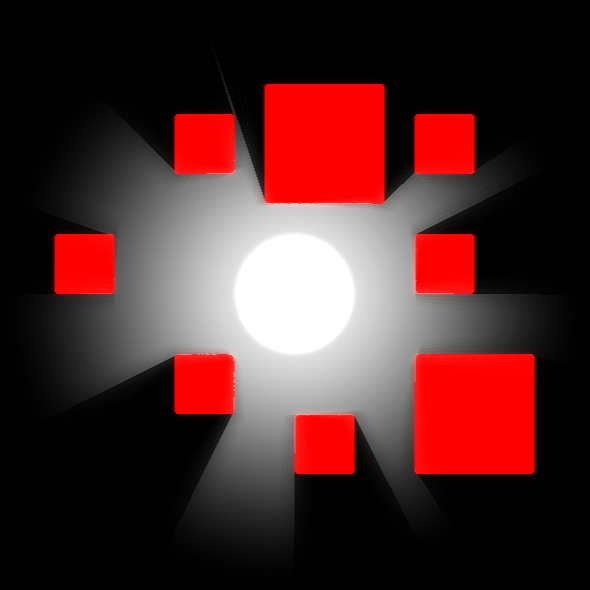
\includegraphics[width=\columnwidth]{../testing/assets/rays_example_1.png}
    \end{subfigure}
    \begin{subfigure}[b]{0.3\columnwidth}
    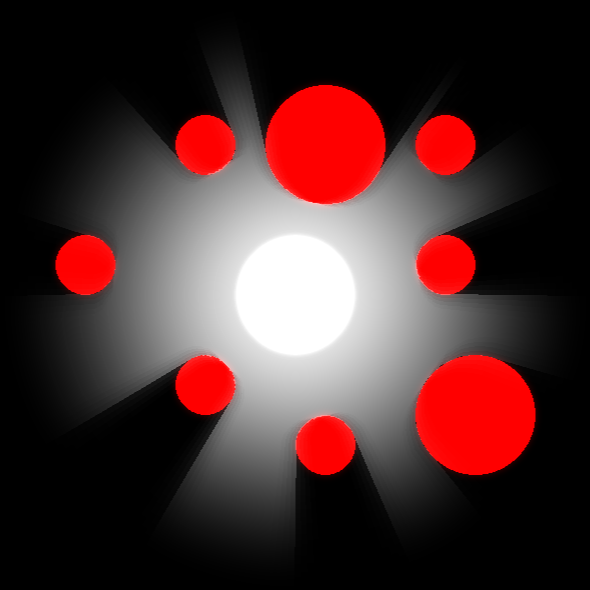
\includegraphics[width=\columnwidth]{../testing/assets/rays_example_2.png}
    \end{subfigure}
    \begin{subfigure}[b]{0.3\columnwidth}
    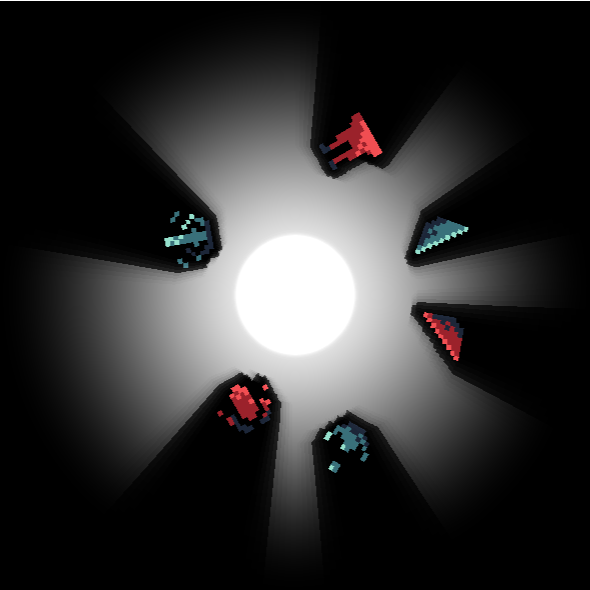
\includegraphics[width=\columnwidth]{../testing/assets/rays_example_3.png}
    \end{subfigure}

    \caption{Shadow mapping algorithm tests (softShadow=0.5, radius=0.5)}
    \label{fig:rays-examples}
\end{figure}

\section{Final Tests}
\subsection{Objective 1}
\subsection{Objective 2}
\subsection{Objective 3}

\section{Videos}

\end{document}